\input{E:/latex/beamer/Boadilla}
\usepackage{csvsimple}
% \usepackage{longtable}     
\title[Tetraquark]{Configurations of heavy tetraquark}
%\titlegraphic{
\includegraphics[scale=1]{group/group.pdf}}
\newcommand{\redtext}[1]{{\color{red} #1}}
\newcommand{\bluetxt}[1]{{\color{blue} #1}}
\newcommand{\Acal}{\mathcal{A}}
\newcommand{\Bcal}{\mathcal{B}}
\begin{document}
\justifying
\begin{frame}
    \titlepage
\end{frame}
\begin{frame}{Contents}
    \tableofcontents
\end{frame}
\section{Motivation}
\begin{frame}{Motivation}
    \begin{figure}[htbp]
        \centering
        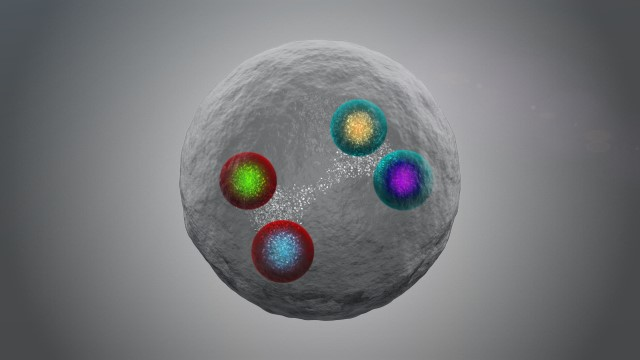
\includegraphics[scale=.4]{LHC-tetraquark.jpg}
        \caption{Charmed existence: conceptual illustration of a tetraquark. (Courtesy: CERN)}
    \end{figure}
\end{frame}
\section{Configuration}
\begin{frame}{Hamiltonian for tetraquark}
    \begin{equation}
        H = \sum_{1}^{4}m_{i} + \sum_{i<j}V_{ij}(r_{ij})
    \end{equation}
    \[
        V_{ij}(r_{ij}) = \lambda_{i}\cdot\lambda_{j}A_{ij} + B_{ij}\frac{1}{m_{i}m_{j}}s_{i}\cdot s_{j}\lambda_{i}\cdot\lambda_{j}
    \]
\end{frame}
\begin{frame}{Diquark-antiquark configuration}{Color-wave function}
    With this configuration, the flavor-wasve function is a trival symmetric function. The color space acting on $\lambda_{i}^{a}\lambda_{j}^{a}$ in a given flavor configuration of tetraquark can be decomposed using the irreducible representation of color SU(3) as
    \begin{equation}\label{Eq: color decomposition}
        3\otimes3\otimes\bar{3}\otimes\bar{3} =\redtext{ \bar{3}\otimes3} + \redtext{6\otimes\bar{6}} + \bar{3}\otimes3 + 6\otimes3.
    \end{equation}
    Color singlet states are given by the first and scond term in the right-hand side of Eq.(\ref{Eq: color decomposition}). The correseponding wave function can be constructed following:
    \begin{align*}
        \ret{\zeta_{1}} & = (Q_{1}Q_{2})^{6}\otimes(\bar{Q}_{3}\bar{Q}_{4})^{\bar{6}} & \ret{\zeta_{2}} & = (Q_{1}Q_{2})^{\bar{3}}\otimes(\bar{Q}_{3}\bar{Q_{4}})^{3}
    \end{align*}
    
\end{frame}
\begin{frame}{Spin-wave function}
    The spin space of tetraquark with diquark-antidiquark configuration can be expressed as $V_{\frac{1}{2}}\otimes V_{\frac{1}{2}}\otimes V_{\frac{1}{2}}\otimes V_{\frac{1}{2}}$, decomposed into the direct sum of the following parts:
    \begin{equation}
        V_{1/2}\otimes V_{1/2}\otimes V_{1/2}\otimes V_{1/2} = V_{0}\otimes V_{0} \oplus V_{0}\otimes V_{1} \oplus V_{1}\otimes V_{0} \oplus V_{1}\otimes V_{1}
    \end{equation}


    \begin{itemize}
        \item Total spin $S=0$ from $V_{0}\otimes V_{0}$
    \end{itemize}
    The correseponding bases are given following:
    \begin{align}
        \chi^{00}_{0} & = \frac{1}{\sqrt{2}}\ret{\uparrow\downarrow-\downarrow\uparrow}\otimes\frac{1}{\sqrt{2}}\ret{\uparrow\downarrow-\downarrow\uparrow}                                                                                                                                                                                                                            \\
        \chi^{11}_{0} & = \frac{1}{\sqrt{3}}\squarebk{\ret{\uparrow\uparrow}\otimes\ret{\downarrow\downarrow}} + \frac{1}{\sqrt{3}}\squarebk{\ret{\downarrow\downarrow}\otimes\ret{\uparrow\uparrow}} - \frac{1}{\sqrt{3}}\squarebk{\frac{1}{\sqrt{2}}(\ret{\uparrow\downarrow}+\ret{\downarrow\uparrow})\otimes\frac{1}{\sqrt{2}}(\ret{\uparrow\downarrow}+\ret{\downarrow\uparrow})}
    \end{align}
\end{frame}
\begin{frame}{Spin-wave function}
    Here, we define the spinors:
    \begin{align}
        \ret{\uparrow}             & =
        \begin{pmatrix}
            1 \\
                0
        \end{pmatrix} &
        \ret{\downarrow}           & =
        \begin{pmatrix}
            0 \\
            1
        \end{pmatrix}.
    \end{align}
    \begin{itemize}
        \item $S=1$ from $V_{1}\otimes V_{1}$, \redtext{$V_{1}\otimes V_{0}$, $V_{0}\otimes V_{1}$}
    \end{itemize}
    \begin{align}
        \ret{\chi^{11}_{1}}           & = \frac{1}{\sqrt{2}}\squarebk{\frac{1}{\sqrt{2}}(\ret{\uparrow\downarrow}+\ret{\downarrow\uparrow})\otimes\ret{\uparrow\uparrow}}-\frac{1}{\sqrt{2}}\squarebk{\ret{\uparrow\uparrow}+\frac{1}{\sqrt{2}}(\ret{\uparrow\downarrow}+\ret{\downarrow\uparrow})} \\
        \redtext{\ret{\chi^{10}_{1}}} & = \ret{\uparrow\uparrow}\otimes\frac{1}{\sqrt{2}}(\ret{\uparrow\downarrow}-\ret{\downarrow\uparrow})\ (\text{Antisymmetry})      \\
        \redtext{\ret{\chi^{01}_{1}}} & = \frac{1}{\sqrt{2}}(\ret{\uparrow\downarrow}-\ret{\downarrow\uparrow})\otimes\ret{\uparrow\uparrow}\ (\text{Antisymmetry})
    \end{align}
\end{frame}
\begin{frame}{Spin-wave function}
    \begin{itemize}
        \item $S=2$ from $V_{1}\otimes V_{1}$
    \end{itemize}
    \begin{equation}
        \ret{\chi^{11}_{2}} = \ret{\uparrow\uparrow}\otimes\ret{\uparrow\uparrow}
    \end{equation}
    \begin{thebibliography}
        \beamertemplatetextbibitems
        %\cite{Park:2013fda}
        \bibitem{Park:2013fda}
        W.~Park and S.~H.~Lee,
        %``Color spin wave functions of heavy tetraquark states,''
        Nucl. Phys. A \textbf{925}, 161-184 (2014)
        %doi:10.1016/j.nuclphysa.2014.02.008
        [\href{https://arxiv.org/abs/1311.5330}{arXiv:1311.5330 [nucl-th]}].
        %16 citations counted in INSPIRE as of 09 Mar 2021
        %\cite{Liu:2019zuc}
    \bibitem{Liu:2019zuc}
    M.~S.~Liu, Q.~F.~L\"u, X.~H.~Zhong and Q.~Zhao,
    %``All-heavy tetraquarks,''
    Phys. Rev. D \textbf{100}, no.1, 016006 (2019)
    %doi:10.1103/PhysRevD.100.016006
    [\href{https://arxiv.org/abs/1901.02564v4}{arXiv:1901.02564 [hep-ph]}].
%51 citations counted in INSPIRE as of 10 Mar 2021
    \end{thebibliography}
\end{frame}
\begin{frame}{The matrix elements of $S_{i}\cdot S_{j}$}
    \begin{table}[htbp]\tiny
        \begin{tabular}{cccc}
            \toprule[1pt]
            $S_{i}\cdot S_{j}$ & $\left\{\ret{\chi^{11}_{0}},\ \ret{\chi^{00}_{0}}\right\}$ & $\curlbk{\ret{\chi^{11}_{2}}}$ & $\curlbk{\ret{\chi^{10}_{1}},\ret{\chi^{11}_{1}},\ \ret{\chi^{01}_{1}}}$ \\\midrule
            $S_{1}\cdot S_{2}$ & $\begin{pmatrix}1/4 & 0\\0 & -3/4\end{pmatrix}$                               & $1/4$                          & $\begin{pmatrix}0 & 0 & 0\\0 & 1/4 &0\\0&0&-3/4 \end{pmatrix}$                                             \\
            $S_{1}\cdot S_{3}$ & $\begin{pmatrix}-1/2&-\sqrt{3}/4\\-\sqrt{3}/4&0\end{pmatrix}$                               & $1/4$                          & $\begin{pmatrix}0&-\sqrt{2}/4&1/4\\-\sqrt{2}/4&\bluetxt{1/4}&\sqrt{2}/4\\-1/4&\sqrt{2}/4&0\end{pmatrix}$                                             \\
            $S_{1}\cdot S_{4}$ & $\begin{pmatrix}-1/2&\sqrt{3}/4\\\sqrt{3}/4&0 \end{pmatrix}$                               & $1/4$                          & $\begin{pmatrix}0&\sqrt{2}/4&-1/4\\\sqrt{2}/4&\bluetxt{-1/4}&\sqrt{2}/4\\-1/4&\sqrt{2}/4&0\end{pmatrix}$                                             \\
            $S_{2}\cdot S_{3}$ & $\begin{pmatrix}-1/2&\sqrt{3}/4\\\sqrt{3}/4&0\end{pmatrix}$                               & 1/4                            & $\begin{pmatrix}0&-\sqrt{2}/4&-1/4\\-\sqrt{2}/4&-1/4&-\sqrt{2}/4\\-1/4&-\sqrt{2}/4&0\end{pmatrix}$                                             \\
            $S_{2}\cdot S_{4}$ & $\begin{pmatrix}-1/2&-\sqrt{3}/4\\-\sqrt{3}/4&0\end{pmatrix}$                               & $1/4$                          & $\begin{pmatrix}-3/4&0&0\\0&1/4&0\\0&0&1/4\end{pmatrix}$                                             \\
            $S_{3}\cdot S_{4}$ & $\begin{pmatrix}1/4&0\\0&-3/4\end{pmatrix}$                               & $1/4$                          & $\begin{pmatrix}-3/4&0&0\\0&1/4&0\\0&0&1/4\end{pmatrix}$
            \\\bottomrule[1pt]
        \end{tabular}
        \caption{Matrix elements of $S_{i}\cdot S_{j}$}
    \end{table}
\end{frame}
\begin{frame}{The matrix elements of $\lambda_{i}^{a}\lambda_{j}^{a}$}
    \begin{table}[htbp]
        \begin{tabular}{ccc}
            \toprule[1pt]
            $\lambda_{i}^{a}\lambda_{j}^{a}$                                & $(q_{1}q_{2})^{6}(\bar{q}\bar{q})^{\bar{6}},\ (q_{1}q_{2})^{\bar{3}}(\bar{q}\bar{q})^{3}$ & $(q_{1}\bar{q}_{3})^{8}(q_{2}\bar{q}_{4})^{8},\ (q_{1}\bar{q}_{3})^{1}(\bar{q}\bar{q})^{1}$ \\\midrule
            $\lambda_{1}^{a}\lambda_{2}^{a}=\lambda_{3}^{a}\lambda_{4}^{a}$ & $\begin{pmatrix}4/3&0\\0&-8/3\end{pmatrix}$                                                              & $\begin{pmatrix}-4/3 & 4\sqrt{2}/3\\4\sqrt{2}/3 & 0\end{pmatrix}$                                                                \\
            $\lambda_{1}^{a}\lambda_{3}^{a}=\lambda_{2}^{a}\lambda_{4}^{a}$ & $\begin{pmatrix}-10/3&-2\sqrt{2}\\-2\sqrt{2}&-4/3\end{pmatrix}$     & $\begin{pmatrix} 2/3 & 0\\0&-16/3\end{pmatrix}$                                                                                                                                                       \\
            $\lambda_{1}^{a}\lambda_{4}^{a}=\lambda_{2}^{a}\lambda_{3}^{a}$ & $\begin{pmatrix}-10/3&2\sqrt{2}\\2\sqrt{2}&-4/3\end{pmatrix}$ & $\begin{pmatrix}-14/3 & -4\sqrt{2}/3\\-4\sqrt{2}/3 & 0 \end{pmatrix}$
            \\\bottomrule[1pt]
        \end{tabular}
        \caption{The matrix elements of $\lambda_{i}^{a}\lambda_{j}^{a}$}
    \end{table}
\end{frame}
\begin{frame}{Wave function of tetraquark with diquark-antidiquark configuration}
    The total wave function of the tetraquark is the direct product of space, flavor, color and spin wave function, i.e.,
    \begin{equation}
        \ret{\psi} = \ret{\psi_{\text{space}}}\ret{\psi_{\text{flavor}}}\ret{\psi_{\text{color}}}\ret{\psi_{\text{spin}}}  .
    \end{equation}
    Since we consider the groud state of tetraquark, the spatial wave function is symmetry. The configurations classified by $J^{PC}$ within Pauli exclusion principle are listed following.

\end{frame}
\begin{frame}{Wave function of tetraquark with diquark-antidiquark configuration}
    \begin{table}[htbp]
        \begin{tabular}{l|c|c}
            \toprule[1pt]
            \multicolumn{2}{c}{Existence} & Non-eistence                                                                                                         \\\midrule
            $0^{++}$                      & $\ret{(cc)^{6}_{0}(\bar{c}\bar{c})^{\bar{6}}_{0}}_{0}$, $\ret{(cc)_{1}^{\bar{3}}(\bar{c}\bar{c})^{3}_{1}}_{0}$ & --- \\[10pt]
            $1^{+-}$                      & $\ret{(cc)^{\bar{3}}_{1}(\bar{3}\bar{3})_{1}^{3}}_{1}$                                                         & ~   \\[10pt]
            $2^{++}$                      & $\ret{(cc)_{1}^{\bar{3}}(\bar{c}\bar{c})_{1}^{3}}_{2}$                                                         & ---
            \\\bottomrule[1pt]
        \end{tabular}
        \caption{Configurations of tetraquark with different $J^{PC}$}
    \end{table}
\end{frame}
\begin{frame}{The mass splitting in hyperfine potential}
    \begin{itemize}
        \item $0^{++}$
    \end{itemize}
    \begin{align}
         &
        \begin{pmatrix}
            \Inner{\zeta_{1}}{\lambda_{i}\cdot\lambda_{j}}{\zeta_{1}}\inner{\chi^{00}_{0}}{\chi^{00}_{0}} & \Inner{\zeta_{1}}{\lambda_{i}\cdot\lambda_{j}}{\zeta_{2}}\inner{\chi^{00}_{0}}{\chi^{11}_{0}} \\[10pt]
            \Inner{\zeta_{2}}{\lambda_{i}\cdot\lambda_{j}}{\zeta_{1}}\inner{\chi^{11}_{0}}{\chi^{00}_{0}} & \Inner{\zeta_{2}}{\lambda_{i}\cdot\lambda_{j}}{\zeta_{2}}\inner{\chi^{11}_{0}}{\chi^{11}_{0}}
        \end{pmatrix}\mathcal{A}_{ij} \\[10pt]
         &
        \frac{1}{m_{i}m_{j}}
        \begin{pmatrix}
            \Inner{\zeta_{1}}{\lambda_{i}\cdot\lambda_{j}}{\zeta{1}}\Inner{\chi^{00}_{0}}{S_{i}\cdot S_{j}}{\chi^{00}_{0}}  & \Inner{\zeta_{1}}{\lambda_{i}\cdot\lambda_{j}}{\zeta_{2}}\Inner{\chi^{00}_{0}}{S_{i}\cdot S_{j}}{\chi^{11}_{0}} \\[10pt]
            \Inner{\zeta_{2}}{\lambda_{i}\cdot\lambda_{j}}{\zeta_{1}}\Inner{\chi^{11}_{0}}{S_{i}\cdot S_{j}}{\chi^{00}_{0}} & \Inner{\zeta_{2}}{\lambda_{i}\cdot\lambda_{j}}{\zeta_{2}}\Inner{\chi^{11}_{0}}{S_{i}\cdot S_{j}}{\chi^{11}_{0}}
        \end{pmatrix}\mathcal{B}_{ij}
    \end{align}

\end{frame}
\begin{frame}{The mass splitting in hyperfine potential}
    \begin{multline}
        V^{0^{++}} =
        (\Acal_{12}+\Acal_{34})\begin{pmatrix}
            4/3 & 0    \\
            0   & -8/3
        \end{pmatrix}
        + (\Acal_{13}+\Acal_{24}+\Acal_{14}+\Acal_{23})
        \begin{pmatrix}
            -10/3 & 0    \\
            0     & -4/3
        \end{pmatrix}\\
        +\frac{\Bcal_{12}+\Bcal_{34}}{m_{c}m_{c}}
        \begin{pmatrix}
            -1 & 0    \\
            0  & -2/3
        \end{pmatrix}
        +\frac{\Bcal_{13}+\Bcal_{24}+\Bcal_{14}+\Bcal_{23}}{m_{\bar{c}}m_{\bar{c}}}
        \begin{pmatrix}
            0          & \sqrt{6}/2 \\
            \sqrt{6}/2 & 2/3
        \end{pmatrix}
    \end{multline}
    \begin{itemize}
        \item $1^{+-}$
    \end{itemize}
    \begin{multline}
        V^{1^{+-}} = (\Acal_{12}+\Acal_{34})\bk{-\frac{8}{3}} + (\Acal_{13}+\Acal_{24}+\Acal_{14}+\Acal_{23})\bk{-\frac{4}{3}}\\
        +\frac{\Bcal_{12}+\Bcal_{34}}{m_{c}m_{c}}\bk{-\frac{2}{3}} +\frac{ (\Bcal_{13}+\Bcal_{24}+\Bcal_{14}+\Bcal_{23})}{m_{\bar{c}}m_{\bar{c}}}\bk{\frac{2}{3}}
    \end{multline}
\end{frame}
\begin{frame}{The mass splitting in hyperfine potential}
    \begin{itemize}
        \item $2^{++}$
    \end{itemize}
    \begin{multline}
        V^{2++} = (\Acal_{12}+\Acal_{34})\bk{-\frac{8}{3}} + (\Acal_{13}+\Acal_{24}+\Acal_{14}+\Acal_{23})\bk{-\frac{4}{3}}\\
        +\frac{\Bcal_{12}+\Bcal_{34}}{m_{c}m_{c}}\bk{-\frac{2}{3}} + \frac{\Bcal_{13}+\Bcal_{24}+\Bcal_{14}+\Bcal_{23}}{m_{\bar{c}}m_{\bar{c}}}\bk{-\frac{1}{3}}
    \end{multline}
\end{frame}
\begin{frame}{Extract $\Acal_{13}$ and $\Bcal_{13}$}
    The Hamiltonian for charmonium is given by
    \begin{equation}
        H_{c\bar{c}} = \bk{\sum_{i=1}^{2}m_{i}+T_{i}} + V_{13},
    \end{equation}
    where $V_{13}=\lambda_{1}\cdot\lambda_{3}A(r_{13})+\frac{B(r_{13})}{m_{1}m_{3}}S_{1}\cdot S_{3}\lambda_{1}\cdot\lambda_{3}$. Within bases $\curlbk{\ret{c\bar{c}}^{1}_{0},\ \ret{c\bar{c}}^{1}_{1}}$, we have
    \begin{align}
        M_{\eta_{c}} & = -\frac{16}{3}\Acal_{13} + 4\Bcal_{13}\frac{1}{m_{c}^{2}} + 2m_{c}       \\
        M_{J/\psi}   & = -\frac{16}{3}\Acal_{13}-\frac{4}{3}\Bcal_{13}\frac{1}{m_{c}^{2}}+2m_{c}
    \end{align}
\end{frame}
\begin{frame}{Extract $\Acal_{12}$ and $\Bcal_{12}$}
    $\Acal_{12}$ and $\Bcal_{12}$ can be extracted from Hamiltonian governing doubly heavy baryon with components $c(1)c(2)q(3)$. The spin of component $c(1)c(2)$ only is $\redtext{S_{cc}=1}$ because the irreducible color representation $\bar{3}$ is antisymmetry. So the spin of double baryons we consider are $S=\frac{3}{2}$ and $S=\frac{1}{2}$. The spin eigenstates of $ccq$ can be written as 
    \begin{equation}\label{Eq:spineigen}
        \ret{(cc)_{1},q_{\frac{1}{2}};\frac{3}{2}},\ \ret{(cc)_{1},q_{\frac{1}{2}};\frac{1}{2}}.
    \end{equation}


    The corresponding Hamiltonian is
    \begin{multline}\label{Eq:Hamccq}
        H = \sum_{i=1}^{3}\bk{m_{i}+T_{i}} + A_{12}\lambda_{1}\cdot\lambda_{2} + A_{13}\lambda_{1}\cdot\lambda_{3} + A_{23}\lambda_{2}\cdot\lambda_{3}\\
        + \frac{B_{12}}{m_{c}m_{c}}\lambda_{1}\cdot\lambda_{2}S_{1}\cdot S_{2} + \frac{B_{13}}{m_{c}m_{q}}\lambda_{1}\cdot\lambda_{3}S_{1}\cdot S_{3} + \frac{B_{23}}{m_{c}m_{q}}\lambda_{2}\cdot\lambda_{3}S_{2}\cdot S_{3}
    \end{multline}
\end{frame}
\begin{frame}{Extract $\Acal_{12}$ and $\Bcal_{12}$}
    For baryon, the color singlet function is
    \begin{equation}
        \zeta = \frac{1}{\sqrt{6}}\bk{rgb-rbg+gbr-grb+brg-bgr}
    \end{equation}
    \begin{thebibliography}
        \beamertemplatetextbibitems
            %\cite{Xiao:2013xi}
            \bibitem{Xiao:2013xi}
            L.~Y.~Xiao and X.~H.~Zhong,
            %``$\Xi$ baryon strong decays in a chiral quark model,''
            %Phys. Rev. D \textbf{87}, no.9, 094002 (2013)
            %doi:10.1103/PhysRevD.87.094002
            [\href{https://arxiv.org/abs/1302.0079v2}{arXiv:1302.0079 [hep-ph]}].
%27 citations counted in INSPIRE as of 09 Mar 2021
    \end{thebibliography}
    The matrix elements $\langle\lambda_{i}\cdot\lambda_{j}\rangle$ in this basis are given following:
    \[
        \langle\lambda_{1}\cdot\lambda_{2}\rangle = \langle\lambda_{1}\cdot\lambda_{3}\rangle = \langle\lambda_{2}\cdot\lambda_{3}\rangle = \frac{-8}{3}.
    \]


    However, the bases Eq.(\ref{Eq:spineigen}) are not suitable for calculating the expectations of $S_{1}\cdot S_{3}$ and $S_{2}\cdot S_{3}$, because The paremeters $A_{13}(B_{13})$ and $A_{23}(B_{23})$ stand for the couple of $c(1)q$ and $c(2)q$, respectively.
\end{frame}
\begin{frame}{Extract $\Acal_{12}$ and $\Bcal_{12}$}
 A change from basis $\ret{(S_{c},S_{c})S_{cc},S_{q};S}$ to $\ret{S_{c},(S_{c},S_{q})S}$ can be accomplished in following way:
    \begin{multline}\label{Eq:spin decomposition}
        \ret{S_{c},(S_{c},S_{q})S_{cq};S} =
        \sum_{S_{cc}=|S_{c}-S_{c}|}^{S_{c}+S_{c}}(-1)^{S_{c}+S_{c}+S_{q}+S}\sqrt{2S_{cc}+1}\sqrt{2S_{cq}+1}\times\\
        \begin{Bmatrix}
            S_{c} & S_{c} & S_{cc} \\
            S_{q} & S     & S_{cq}
        \end{Bmatrix}
        \ret{(S_{c},S_{c})S_{cc},S_{q};S}
    \end{multline}
    For $\ret{(S_{c2},S_{c1})S_{cc},S_{q};S}$, we have the relationship:
    \begin{align*}
        \ret{(S_{c1},S_{c2})S_{cc},S_{q};S} 
        &= (-1)^{S_{c1c2}-S_{c1}-S_{c2}}\ret{(S_{c2},S_{c1})S_{cc},S_{q};S}\\
        &=\ret{(S_{c2},S_{c1})S_{cc},S_{q};S}
    \end{align*}
\end{frame}
\begin{frame}{Extract $\Acal_{12}$ and $\Bcal_{12}$}
    With Eq.(\ref{Eq:spin decomposition}),
    \begin{align}
        \ret{(cc)_{1},q_{\frac{1}{2}};\frac{3}{2}} 
        &= \ret{c_{\frac{1}{2}},(cq)_{1};\frac{3}{2}} \\
        \ret{(cc)_{1},q_{\frac{1}{2}};\frac{1}{2}} 
        &= \frac{\sqrt{3}}{2}\ret{c_{\frac{1}{2}},(cq)_{0};\frac{1}{2}} + \frac{1}{2}\ret{c_{\frac{1}{2}},(cq)_{1};\frac{1}{2}}
    \end{align}
    
    
\end{frame}
\begin{frame}{Extract $\Acal_{12}$ and $\Bcal_{12}$}
    \begin{table}[htbp]
        \begin{tabular}{@{}l|c|c|c|c@{}}
            \toprule[1pt]
            $S_{i}\cdot S_{j}$ & $\ret{(cc)_{1},q_{\frac{1}{2}};\frac{3}{2}}$ & $\ret{c_{\frac{1}{2}},(cq)_{1};\frac{3}{2}}$   & $\ret{c_{\frac{1}{2}},(cq)_{1};\frac{1}{2}}$ & $\ret{c_{\frac{1}{2}},(cq)_{0};\frac{1}{2}}$               \\\midrule
            $S_{1}\cdot S_{2}$                       & $\frac{1}{4}$        & ---  & --- & ---\\[10pt]
            $S_{1}\cdot S_{3}$                       & ---        & $\frac{1}{4}$ & $\frac{1}{4}$ & $-\frac{3}{4}$\\[10pt]
            $S_{2}\cdot S_{3}$                       & ---        & $\frac{1}{4}$ & $\frac{1}{4}$ & $-\frac{3}{4}$
            \\\bottomrule[1pt]
        \end{tabular}
        \caption{The expectations of $S_{i}\cdot S_{j}$}
    \end{table}
\end{frame}
\begin{frame}{Extract $\Acal_{12}$  and $\Bcal_{12}$}
    We adopt the masses of doubly heavy baryons $\Omega_{cc}$ and $\Omega_{cc}^{*}$.
    
    \begin{table}[htbp]
        \csvautotabular{Expoparas.csv}
    \caption{Parameters}
    \end{table}
    \begin{thebibliography}
        \beamertemplatetextbibitems
        %\cite{Mathur:2018rwu}
        \bibitem{Mathur:2018rwu}
        N.~Mathur and M.~Padmanath,
        %``Lattice QCD study of doubly-charmed strange baryons,''
        Phys. Rev. D \textbf{99}, no.3, 031501 (2019)
        doi:10.1103/PhysRevD.99.031501
        [\href{https://arxiv.org/abs/1807.00174}{arXiv:1807.00174 [hep-lat]}].
        %20 citations counted in INSPIRE as of 09 Mar 2021
    \end{thebibliography}
    The codes for these calculations can be downloaded from this URL: \url{https://github.com/PLHzzj/zhang.git}
\end{frame}
\begin{frame}{Mass spectra}
    \begin{table}[htbp]
        \csvautotabular{MassSpectra.csv}
    \caption{Mass spectra (unit: MeV)}
    \end{table}
\end{frame}
\end{document}








